\subsection{Iteration 1: Uganda Coach Visit}

% How was this iteration designed?

Following the service design sequencing, the first iteration had a very broad scope and truly is a service design iteration: "From your perspective, what is it like being a coach?\footnote{A coach meaning either a Community Based Trainer (carrying out all the trainings), or a YoungDrive coach, depending on who was asked the question.}". Starting the project had the goal of getting a preliminary understanding of all important aspects, and build relationships with all stakeholders.

%The project started with a startup meeting with Shifteh from Plan International in Kampala, together with Iliana. From there, I did research and met with Grameen Foundation and Designers Without Borders, before going to Tororo to research "What's it like being a YoungDrive coach?", and determining how advanced an app could be to solve challenges that the coaches face.

All insights depended heavily on interviews with all the stakeholders  (2 with Plan International, 3 with YoungDrive), and local experts (1 visit each at Grameen Foundation and Designers without Borders, 1 workshop with Mango Tree), since no Interactions with users had been made yet. Also, knowledge and connections were made with the Kampala technology scene as much as possible, which was benefited by working at the technology hub and co-working space Hive Colab.

Ideation was about creating a questionnaire guide for the interviews, a co-creation workshop using "Customer Journey Map", and identifying how the app test should be designed to test their existing knowledge (and be informed of the design preferences of the YoungDrive app).

Trigger material was the finished questionnaire guide (constructed with Expedition Mondial) a written plan for the co-creation workshop ("A day as a coach"), and a written plan for testing the quiz app Quizoid \citep{quizoid} and the language learning app Duolingo \citep{duolingo}, and a schedule for the interactions.

The interactions were focused on design ethnology, getting to know and learn from people in a different culture, namely the coaches. The focus was on their needs, motivations, and environment. To understand these, four days were spent in Tororo, with one day of travel. There were four face-to-face interviews,
one meeting with Plan, one meeting with the local partners, two workshops, one coach stay-over, and two youth session visits (one of the youth sessions are observable via figure \ref{fig:youthsession}.

\begin{figure}[h]
    \centering
    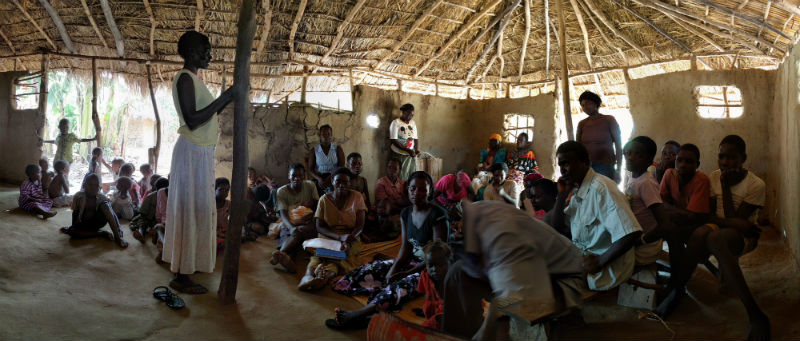
\includegraphics[width=0.7\textwidth]{youthsessionSmall.jpg}
    \caption{Photograph from the location where one of the youth sessions were held. Here, a YoungDrive coach in Tororo teaches youth in basic sales and marketing.}
    \label{fig:youthsession}
\end{figure}

\subsubsection{Customer Journey Map: "A Day As a Coach"}
The first workshop had the tree interviewed coaches as participants. See figure \ref{fig:cjm}. A Customer Journey Map would be created, with the purpose to understand all activities involving “A day as a coach”. The structure of the timeline was: “Before”, “During”, and “After” a youth session. Too understand how these activities differentiated between different coaches, three Personas were co-created based on the previously discovered types of coaches: "the ideal coach" ("John"), "the realistic coach" ("Joan"), and "the challenged coach" ("Suzan").

    \begin{figure}[h]
        \centering
        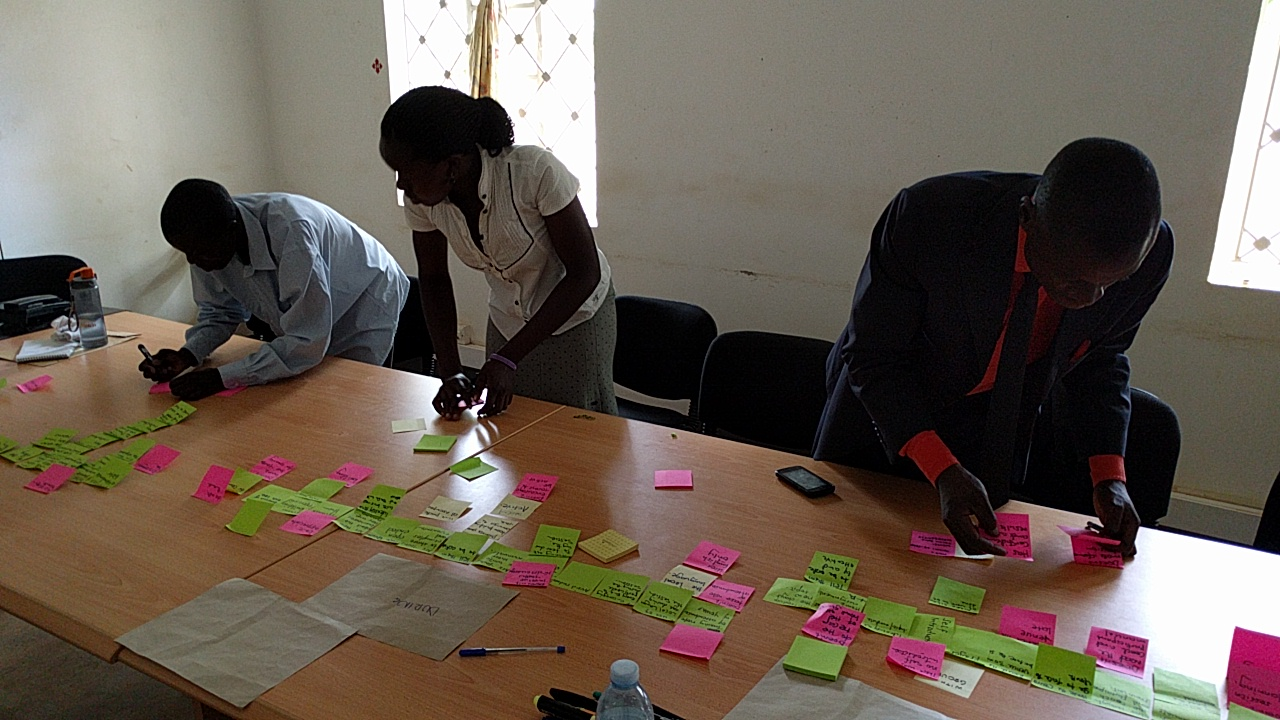
\includegraphics[width=0.7\textwidth]{cjmWorkshop.jpg}
        \caption{Two local project leaders and one coach mapping out the activities a coach does before, during and after hosting a youth session, in what is called a Customer Journey Map.}
        \label{fig:cjm}
    \end{figure}
